\subsection{Backdoors and communications with a controlled server}
\label{ssec:backComm}
After a successful \textit{initial access} attack, which deploys techniques (using entry vectors) to gain an initial foothold within an organization's internal network, adversaries usually install some sort of mechanism that allows them to re-access the network externally, so that in the event that the existing connection is lost, they do not lose the access they have already achieved.

\subsubsection{Different types of system connections}
\label{ssec:persistenceTypes}
As mentioned in the book\cite{RTBook}, there are different types of connectivity situations a computer can be in:
\begin{itemize}
\item System exposed to the Internet
\item Internal systems
\begin{itemize}
\item Computer with \underline{direct connection} to the Internet (different kinds of protocols may apply)
\item Computer with connection to the Internet \underline{through a proxy} (credentials usually needed)
\item Computer \underline{without any type of connection} to the Internet (another machine needs to be compromised to be used as an intermediary)
\end{itemize}
\end{itemize}

For each of the systems listed before, distinct types of backdoors should be applied due to having different requirements and advantages. Therefore, it is crucial to perform an analysis on the system, as explained in section \ref{ssec:recon}, before deploying any kind of persistence or backdoor mechanisms. 

Also, when planning to deploy a backdoor, it is always easier the more exposed to the Internet the compromised machine is, because it is more difficult to find abnormal traffic if the computer has little traffic restrictions, like internal systems with a direct connection.

\subsubsection{Using different communication protocols}
\label{sssec:backProt}
A backdoor is often deployed by a program (or a script) that establishes a connection to a remote server, controlled by the attackers. This connection is usually performed discreetly, to avoid alerting the company's security team; and in consequence, the protocol used and the message sent are studied carefully in order to blend better with the enterprise's normal traffic, difficulting its detection.

For many years, the communication between a compromised client and a controlled server was established using a basic TCP connection. But as network security mechanisms became more advanced and plain TCP connections were less and less frequent (most used protocols nowadays use TCP on their core, but have additional functionalities), modern firewalls and other network devices are usually configured to drop simple TCP connections. Hence, new strategies were created to establish communication, and the most used one is called "\textbf{tunneling}".

\paragraph{Technical data about tunneling}

A tunnel allows for the movement of data between different networks using encapsulation, which is a technique that consists in repackaging the traffic data into a different form, to hide the nature of the communication that is run through.

An easy example can be explained with the HTTP protocol since it is known to usually carry data of variable size. As can be seen in figure \ref{img:httprequest}, an HTTP Request message has some headers and a data field. This "entity body" (the data section), can be used to store any type of information and is useful in some request methods like POST, where data is sent to the server.

The amount of information that can be sent in an HTTP Request is not defined by any standard, but it is usually around 2KB and 8KB in GET requests, and can be up to 2GB in POST requests (depending on the server receiving the message). 

HTTP Response messages follow a similar fashion, as the HTTP specification does not impose a specific size limit. That is why the use of this protocol is common when performing encapsulation, as big chunks of data can be stored inside the data field.

\begin{figure}[!ht]
	%\hspace{-1.5cm}
	\centering
	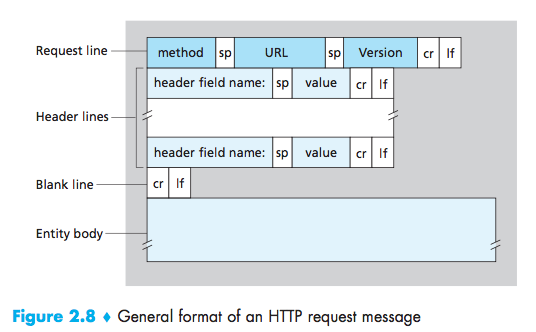
\includegraphics[width=13cm,trim={0 1cm 0 0},clip]{img/http-request-message.png}
	\caption{General format of an HTTP Request message}
	\label{img:httprequest}
\end{figure}

\textbf{Encapsulation} is a technique that has been used for years to allow network communication: it is a fundamental part of the Open Systems Interconnection model (OSI model) and the TCP/IP model. 

The aforementioned models define different abstract layers to organize all protocols that are necessary to establish a connection. Their implementation can be summarized in the following steps:
\begin{enumerate}
\item The computer that sends the message, wraps the information to be sent in the data field of the top layer, and adds this layer protocol's header (first encapsulation). 
\item Then, it encapsulates both header and data into the next layer's protocol data field, and so on. 
\item When the last layer is reached, the computer sends the encapsulated data as 0s and 1s.
\item The computer that receives the message is the one that unwraps every layer to finally obtain the data that is in the most internal layer.
\end{enumerate}

It is important to note that network devices, like firewalls or routers, often unwrap part of the message too, to be able to route it from its origin to its destination (among other purposes). But if the data is sent unencrypted, all devices that receive that message are also able to obtain the sent data.

Continuing with the HTTP message example, this data is later encapsulated in the next layer's protocol: the HTTP Request message is then sent as the data of the TCP/IP packet, and so on until reaching the physical layer, as can be seen in figure \ref{img:osilayers}.

\begin{figure}[!ht]
	%\hspace{-1.5cm}
	\centering
	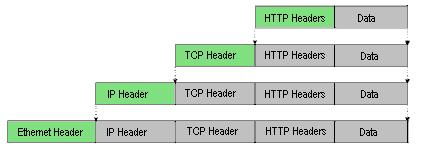
\includegraphics[width=13cm]{img/osilayers}
	\caption{Encapsulation of the different layers}
	\label{img:osilayers}
\end{figure}

\pagebreak
In regular communication, inside the HTTP message, there would be HTTP data. But what if, instead of HTTP information, the HTTP message contains another protocol communication data, like a TCP communication?  Like adding another layer of encapsulation, using this methodology it is possible to establish a plain TCP connection with a remote server, while this connection is being identified by network security systems as a simple HTTP (or HTTPS) connection.

It is worth mentioning that this kind of tunnel, like tunneling a TCP connection through an HTTP communication, generates a high amount of traffic packets in a short time. This is an inconvenience because it can still be detected by security mechanisms (if they look for peaks of traffic), and it can also produce a denial of service to the server receiving the traffic, or to other network tools that analyze it, as sometimes they are not prepared for a high amount of messages.

Tunna\cite{Tunna} is a tool that encapsulates a TCP connection and sends it as HTTP data, which can be seen in figure \ref{img:tunnaEncap}. The wrapping and unwrapping (or encapsulation) of the data is performed by Tunna client and Tunna server, both of which can be set up with a SOCKs\footnotemark proxy to simplify the communication.

\footnotetext{ \textbf{SOCKS}: an Internet protocol that exchanges network packets between a client and server through a proxy server, typically using TCP, and that can be configured in a machine to automatically gather all the Internet traffic (or just a specific applications' traffic) to send it directly through this tunnel.}

\begin{figure}[!ht]
	%\hspace{-1.5cm}
	\centering
	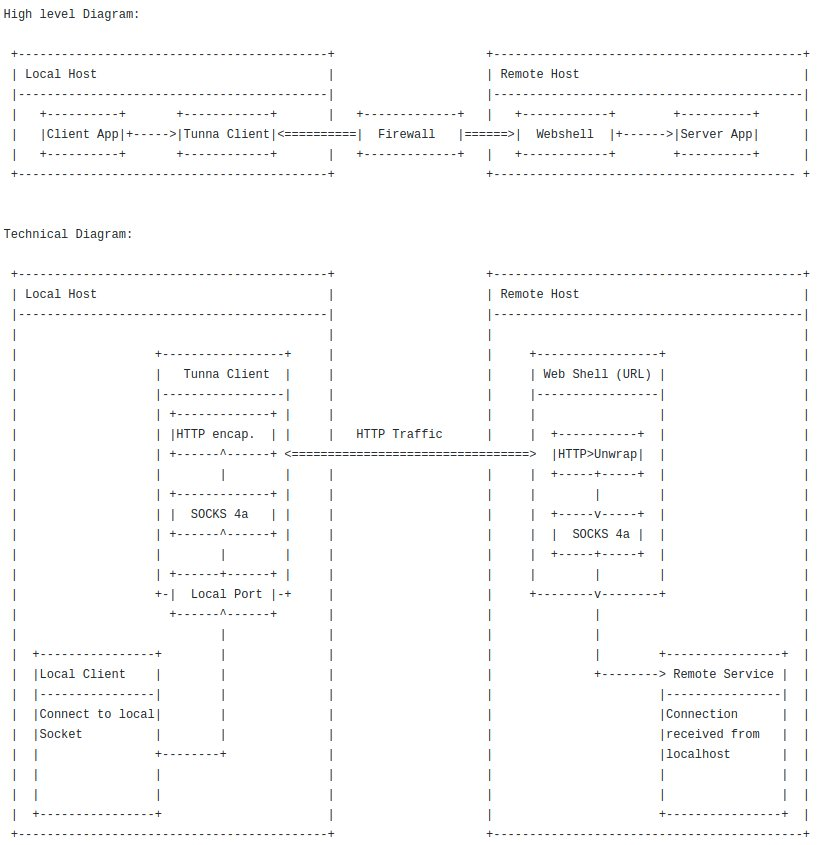
\includegraphics[width=14cm,trim={0 0 0 9cm},clip]{img/tunnaworks}
	\caption{Tunna HTTP encapsulation}
	\label{img:tunnaEncap}
\end{figure}

Finally, there are a few well-known protocols that are commonly used for tunneling like \textit{SSH}, which provides remote administration capabilities; but they are easily spottable by any security mechanism because they are not frequently used from a machine inside an organization to a random server that is on the Internet, or vice versa (usually they are only used inside the same network).

\pagebreak
%\todo[inline]{Si tinc temps i ganes, potser estaria bé posar també un exemple de trafic encapsulat per cada un d'aquests protocols}
\paragraph{Most used protocols in a corporation network}

There are different kinds of protocols that are commonly used within an organization, and for this reason, most of the backdoors work by establishing communication (a tunnel) through one of them:
\begin{itemize}
\renewcommand{\labelitemi}{\localtextbulletone}
\item \textbf{HTTP and HTTPS}: web traffic is by far the most popular, but it is often audited and controlled through various security mechanisms (such as proxies). Also, even though HTTP is almost deprecated through the Internet, it is still used to access resources from within a network.
\item \textbf{DNS}: or \textit{Domain Name System}, is the service used to find machines (and domains) by name instead of by IP. Since machines have names even inside a corporation's networks, it is frequent to find DNS servers inside of an organization. For this reason, critical machines without Internet access through HTTPS, such as internal servers or industrial systems (which technicians avoid exposing to the Internet), sometimes have DNS communication to internal servers, which also communicate to the Internet, and a connection can be created using this method.  

\pagebreak
\item \textbf{ICMP}: the \textit{Internet Control Message Protocol} is the one used in \texttt{ping} requests. Even though it can also be employed to establish a communication to an external server, it is the least reliable protocol as it is easily detected (in fact it is not one of the protocols that generate big volumes of traffic in an organization, as HTTPS and DNS do) and it is pretty common for big corporations to disallow the use of this protocol to external servers. But it can still be an option if all other protocols are not available.
\end{itemize}


\subsubsection{Domains, cryptography and timers}
To end this section, it is important to highlight that there are other decisive elements when setting a backdoor, like the domain to use on the controlled external server, the encryption in the communication between the compromised machine and the external server, and the frequency in which the backdoor program will try to establish a connection.

\paragraph{Domain classification}
When setting a controlled server on the Internet, it is essential to obtain a domain name that is adequate for the environment the victim's machine is in. Domains can be filtered by the company's proxy if it has a reputation (a property set by the proxy's vendor) that is negative, dubious, or it is just not allowed by the company's policies (like "Videogames" or "Movies"). 

Therefore, it is very useful to buy an already classified domain (domains not classified can be problematic as well) that has a good reputation among proxies, being categorized as something harmless like "News" or "Technology".

A good way to buy categorized domains is to check websites with lists of expired domains, like "ExpiredDomains.net"\cite{ExpiredDomainsWeb} and check their reputation in proxy's websites, like Palo Alto\cite{PaloAltoFilteringWeb}. There are also tools to list both the expired domains and their category, like "Domain Hunter"\cite{DomainHunterWeb}.

% \footnotemark\footnotetext{ https://www.expireddomains.net/expired-domains/}
% \footnotemark\footnotetext{ https://urlfiltering.paloaltonetworks.com/}
% \footnotemark\footnotetext{ https://github.com/threatexpress/domainhunter}
\paragraph{Securing communications}
As stated in the previous section \ref{ssec:recon}, web proxies are tools that usually read plain text web requests, even though the communication protocol is HTTPS (that should already have a layer of cryptography). Moreover, other protocols like DNS or ICMP are not encrypted by default.

To protect the information sent to or from the compromised machine, these communications are often encrypted with an algorithm like RC4 (with the key hardcoded into the code or provided in the arguments), thus avoiding raising suspicions when sending commands inside the responses.

\paragraph{Clever timing}
Finally, it should be noted that backdoors are to be used only if the main connection is lost, so they must remain hidden until necessary. If backdoors are being found before using them, the blue team (cybersecurity group) can have more information about which machines are compromised and the mechanisms used by attackers when deploying persistence, so it can compromise the whole operation.

In consequence, it is better to just configure them to make a few connections to the external server every now and then, at random times. Usually, there is a lot of traffic in a network, even in little businesses, so if the backdoor does not stand out, the chances of being discovered before actually using it are reduced to the minimum.

\pagebreak
\subsection{General recommendations when using persistence and backdoors}
\label{ssec:persistenceTips}
In the book\cite{RTBook}, there are listed some guidelines that can help to make the deployment of persistence a little more successful: 
\begin{itemize}
\item Deploy multiple persistences in the same computer
\item Restrict access to the files left by the deployment
\item Create multiple hashes for the same file* 
\item Use multiple deploy origins: different machines, different networks,... 
\item Blend with other files: using similar names to the ones on the folder, or legit system files names, faking metadata (like date), etc.
\item Obfuscation and cipher of the code.
\end{itemize}

* Using multiple file hashes is really interesting, since antimalware solutions do not classify an entire file as malicious, but only its \underline{hash}: an attribute that is calculated using the file data and type.\\ 
When malware is found and identified in a computer, security measures usually look for files with the same hash to delete them, containing the infection. Consequently, changing a bit in the malicious file (like adding spaces or changing variable names) makes it work the same while changing the file hash. So this is a common strategy to avoid all deployed copies being detected easily by security programs.\\

If a backdoor is deployed as well, there are additional tips that can be applied:
\begin{itemize}
\item Use of unusual protocols or methods (like DNS or ICMP)
\item Use different controlled servers or multiple domain names: if a domain is blocked, another one can be used instead
\item Connect at semi-random times
\item Connect using certificates (to prevent other attackers to use the connection)*
\end{itemize}

* An example of this technique is to use public and private keys, like in SSH connections, as it is explained in section \ref{sssec:linuxTools}.